\subsection{Robustness and baseline comparison}
Across the 12 synthetic conditions where the actual Byzantine count and honest coverage satisfy the configured budgets ($f$ and $r$), the robust feasible-set rule achieved zero wrong decisive classifications (0\% FA and 0\% FR) with a mean decisive coverage of 87.52\%, outperforming the fixed-margin baseline (75.63\%) by 11.89 percentage points. A paired cluster bootstrap resampling the 12 condition-level differences with replacement (20,000 draws; fixed pseudorandom seed 718263) yields a 95\% percentile interval of [9.45, 14.56] percentage points. Across these conditions, robust decisive coverage ranges from 79.46\% to 94.29\%, versus 62.63\% to 85.96\% for the fixed-margin baseline. The 11.89-point result is a macro-average over 12 calibrated conditions; the 9.38-point gain reported next is specific to the correlated, radius-four, one-Byzantine focus condition.

\begin{table}[htbp]\centering\footnotesize
\caption{Decisive coverage across the 12 within-budget synthetic conditions (percent). Values are means over 30 seeds per condition; each condition comprises 2,400 events.}\label{tab:twelve}
\begin{tabular}{lrrrr}\toprule
Honest error model&$a$&Actual Byzantine&Robust&Fixed margin\\\midrule
Independent&2&0&94.29&85.21\\
&2&1&94.00&83.42\\
&4&0&90.50&76.38\\
&4&1&87.50&72.58\\
&6&0&85.96&68.83\\
&6&1&84.96&62.62\\
Correlated&2&0&92.04&85.96\\
&2&1&91.25&85.58\\
&4&0&85.08&75.54\\
&4&1&85.04&75.67\\
&6&0&79.46&67.54\\
&6&1&80.12&68.25\\
\bottomrule
\end{tabular}\end{table}




Table~\ref{tab:semantic} details the focus condition (correlated calibrated errors, maximum radius 4, and one Byzantine issuer). The robust rule achieves 85.04\% decisive coverage with zero errors, whereas the fixed-margin rule reaches 75.67\%. Point-estimation baselines (median point and majority center) classify 100\% of events but suffer from 2.10\% FA and 15.29\%--16.30\% FR due to boundary uncertainty. All-source intersection fails on 87.63\% of events and has a marginal 8.64\% FA among truly outside events and 47.55\% FR among truly inside events. Among its rare decisive classifications, all observed decisions in the focus sample were wrong; reporting only marginal rates would obscure this selectivity. Using a 10,000-resample paired bootstrap across the 30 seed groups, the robust rule improves decisive coverage over fixed margins by 9.38 percentage points (95\% CI: $[8.25, 10.54]$ percentage points).



\begin{table}[htbp]\centering\small
\caption{Focus-condition classification results: means over 30 seeds of 80 events each (percent). FA/FR use outside/inside denominators; the other columns use all events.}\label{tab:semantic}
\begin{tabular}{lrrrrr}\toprule
Method&FA&FR&Amb.&Failure&Decisive\\\midrule
Median point claim&2.10&15.29&0&0&100\\
Majority center&2.10&16.30&0&0&100\\
Fixed maximum-radius margin&0&0&24.33&0&75.67\\
All-source intersection&8.64&47.55&0&87.63&12.38\\
Robust feasible set&0&0&14.96&0&85.04\\\bottomrule
\end{tabular}\end{table}

Grouping events by the actual honest-miscoverage count $M$ checks Proposition 1 against the simulated cases. In the focus condition, all 2,400 events satisfy $M = 0 \le r$ with zero observed wrong decisive outcomes. At the seed-group level, the 30 independent seeds yield a one-sided 95\% exact binomial upper bound of 9.50\% on the probability that a seed exhibits at least one wrong decisive outcome; this does not establish a zero population error rate. Under the undercovered error model, the proportion of events satisfying $M \le r$ increases from 52.42\% ($r = 0$) to 62.79\% ($r = 1$) and 73.42\% ($r = 2$). Across all three settings, events satisfying $M \le r$ incurred strictly zero wrong decisive classifications, whereas premise violations ($M > r$) resulted in wrong-decisive rates of 1.31\%, 0.67\%, and 0.47\%, respectively.

\begin{figure}[htbp]\centering
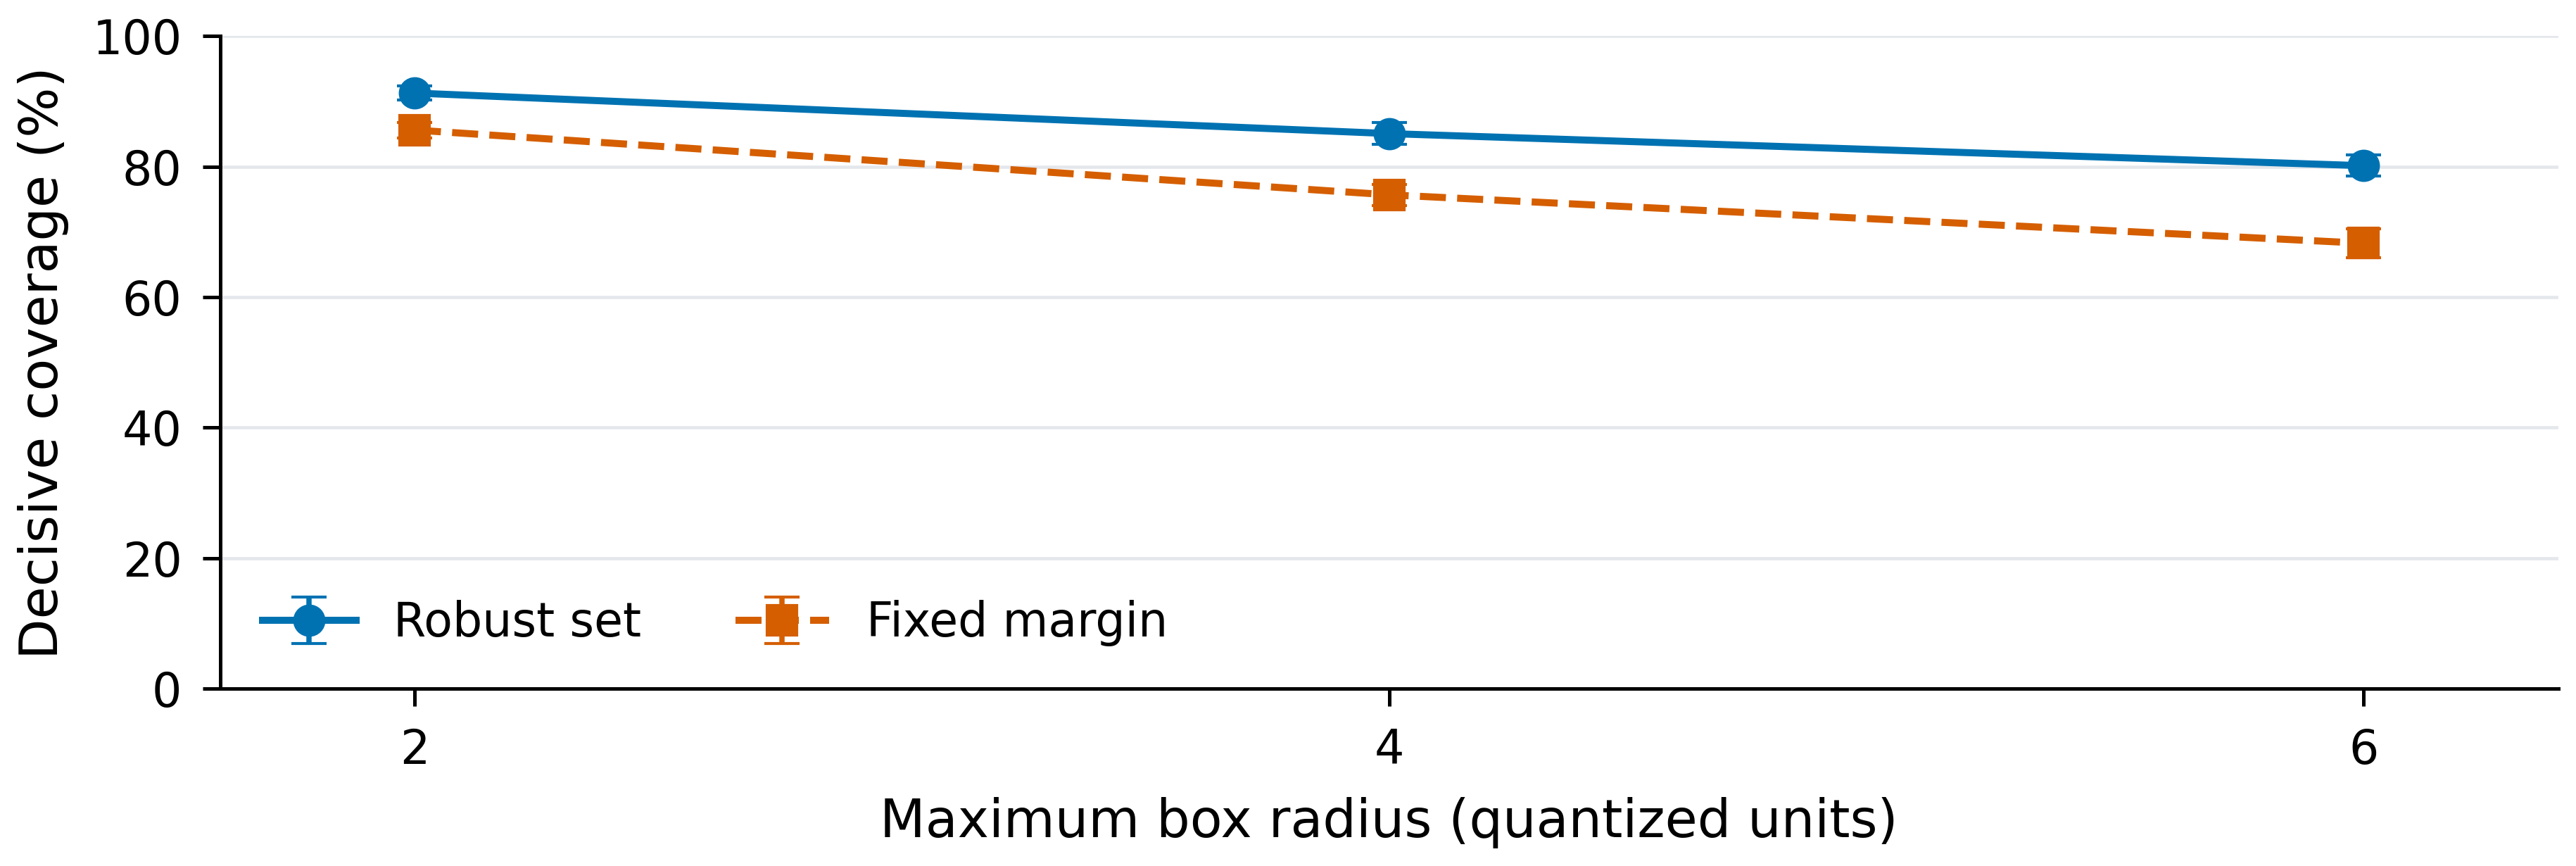
\includegraphics[width=\linewidth]{availability.png}
\caption{Decisive coverage versus maximum uncertainty radius (in quantized units) under correlated calibrated errors with one Byzantine issuer. Error bars denote 95\% confidence intervals across 30 seeds.}\label{fig:availability}
\end{figure}


Figure~\ref{fig:riskcoverage} presents the corresponding risk--coverage operating points for the focus setting. The plotted conditional risk divides wrong decisive outcomes by all decisive classifications, unlike the marginal FA/FR definitions in Table~\ref{tab:semantic}. Since each baseline is tested at one fixed operating point, the figure is an operating-point comparison rather than a continuously tuned risk--coverage curve. For example, all-source intersection achieves only 12.38\% coverage and its 297 decisive decisions are all wrong in the aggregate focus sample; the robust and fixed-margin rules both have zero observed risk at different coverage levels.
\begin{figure}[htbp]\centering
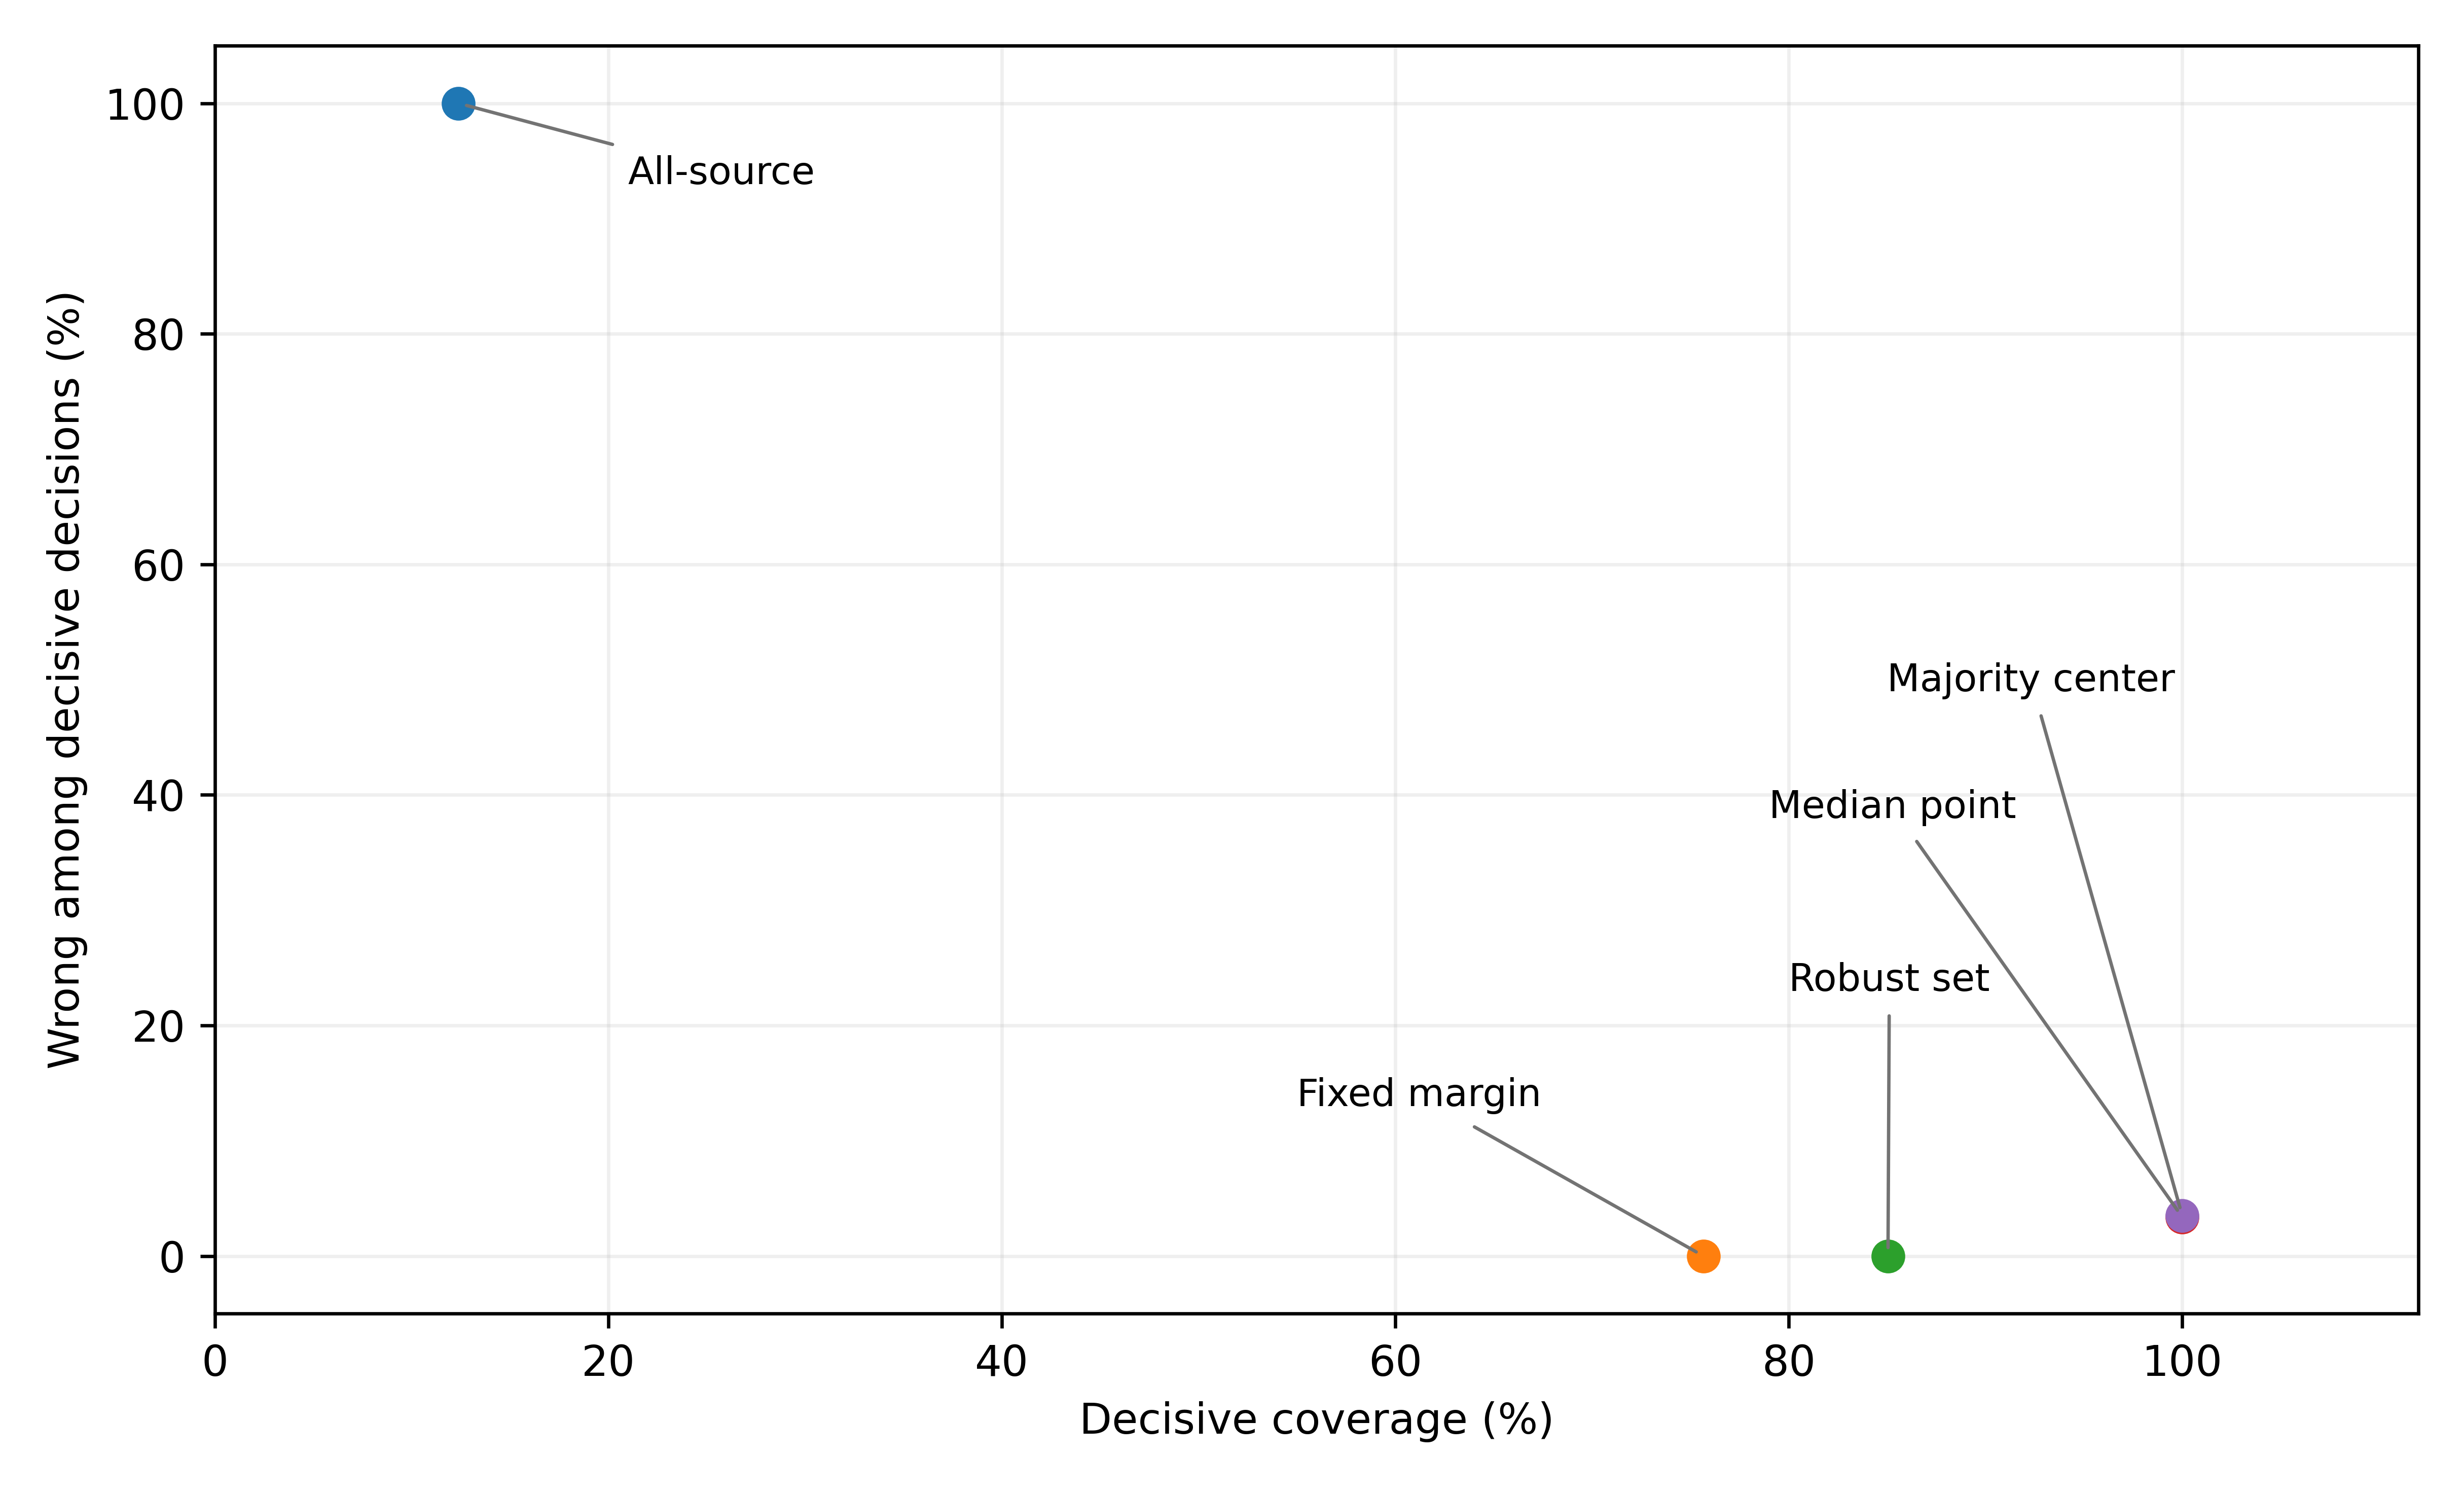
\includegraphics[width=0.92\linewidth]{risk_coverage.png}
\caption{Focus-condition conditional wrong-decision risk versus decisive coverage for five methods; each point uses the aggregate 2,400 generated events. Marginal FA/FR in Table~\ref{tab:semantic} have different denominators.}\label{fig:riskcoverage}
\end{figure}

\subsection{Ablation and out-of-budget stress tests}
Table~\ref{tab:assumption-stress} evaluates system behavior when external assumptions are violated. Under honest-source undercoverage ($M > r$) with one Byzantine issuer, the robust rule experiences 0.23\% FA and 3.41\% FR. When two Byzantine issuers attack a verifier configured for $f = 1$, evidence failure rises to 83.33\% and conditional FA/FR reach 11.62\% and 60.86\%, confirming that the Inconsistent state ($\mathcal{F}_k = \emptyset$) reflects empty threshold support rather than serving as a universal detector for out-of-budget collusion.



\begin{table}[htbp]\centering\small
\caption{Stress conditions violating source assumptions: means over 30 seeds (percent).}\label{tab:assumption-stress}
\begin{tabularx}{\linewidth}{@{}Xrrrr@{}}\toprule
Condition&FA&FR&Evidence failure&Decisive\\\midrule
Honest undercoverage; Byzantine count within budget&0.23&3.41&0&84.92\\
Two actual Byzantine issuers with verifier budget $f=1$&11.62&60.86&83.33&16.67\\\bottomrule
\end{tabularx}\end{table}

Table~\ref{tab:miscoverage} and Figure~\ref{fig:budget} show the paired ablation over the honest-miscoverage budget $r \in \{0, 1, 2\}$ for $n = 5, f = 1$. Because increasing $r$ lowers the support threshold $k = n - f - r$ and expands $\mathcal{F}_k$, it trades decisive coverage for stronger protection against uncalibrated honest misses. Under calibrated evidence, increasing $r$ from 0 to 2 reduces decisive coverage from 85.04\% to 77.46\% while maintaining zero errors. Under undercovered evidence, raising $r$ from 0 to 2 eliminates FA (from 0.23\% to 0\%) and reduces FR from 3.41\% to 0.94\%, with decisive coverage shifting from 84.92\% to 78.50\%.

The UrbanNav trajectory replay shows a similar pattern under simulated multisource errors. Under nominal simulated errors, the robust rule achieves 93.27\% decisive coverage with zero errors, outperforming fixed margins (81.94\%) and avoiding the errors of the median-point baseline (0.29\% FA, 3.12\% FR). Under the $4\times$ common-mode bias stress test, the robust rule maintains low error rates of 0.032\% FA and 0.493\% FR.

\begin{table}[htbp]\centering\small
\caption{Paired ablation over honest-miscoverage allowance ($n=5$, $f=1$, maximum radius four, one Byzantine issuer; percent).}\label{tab:miscoverage}
\begin{tabular}{lrrrr}\toprule
Error model&$r$&FA&FR&Decisive coverage\\\midrule
Calibrated&0&0&0&85.04\\
Calibrated&1&0&0&81.25\\
Calibrated&2&0&0&77.46\\
Undercovered&0&0.23&3.41&84.92\\
Undercovered&1&0&1.79&81.67\\
Undercovered&2&0&0.94&78.50\\\bottomrule
\end{tabular}\end{table}

\begin{figure}[htbp]\centering
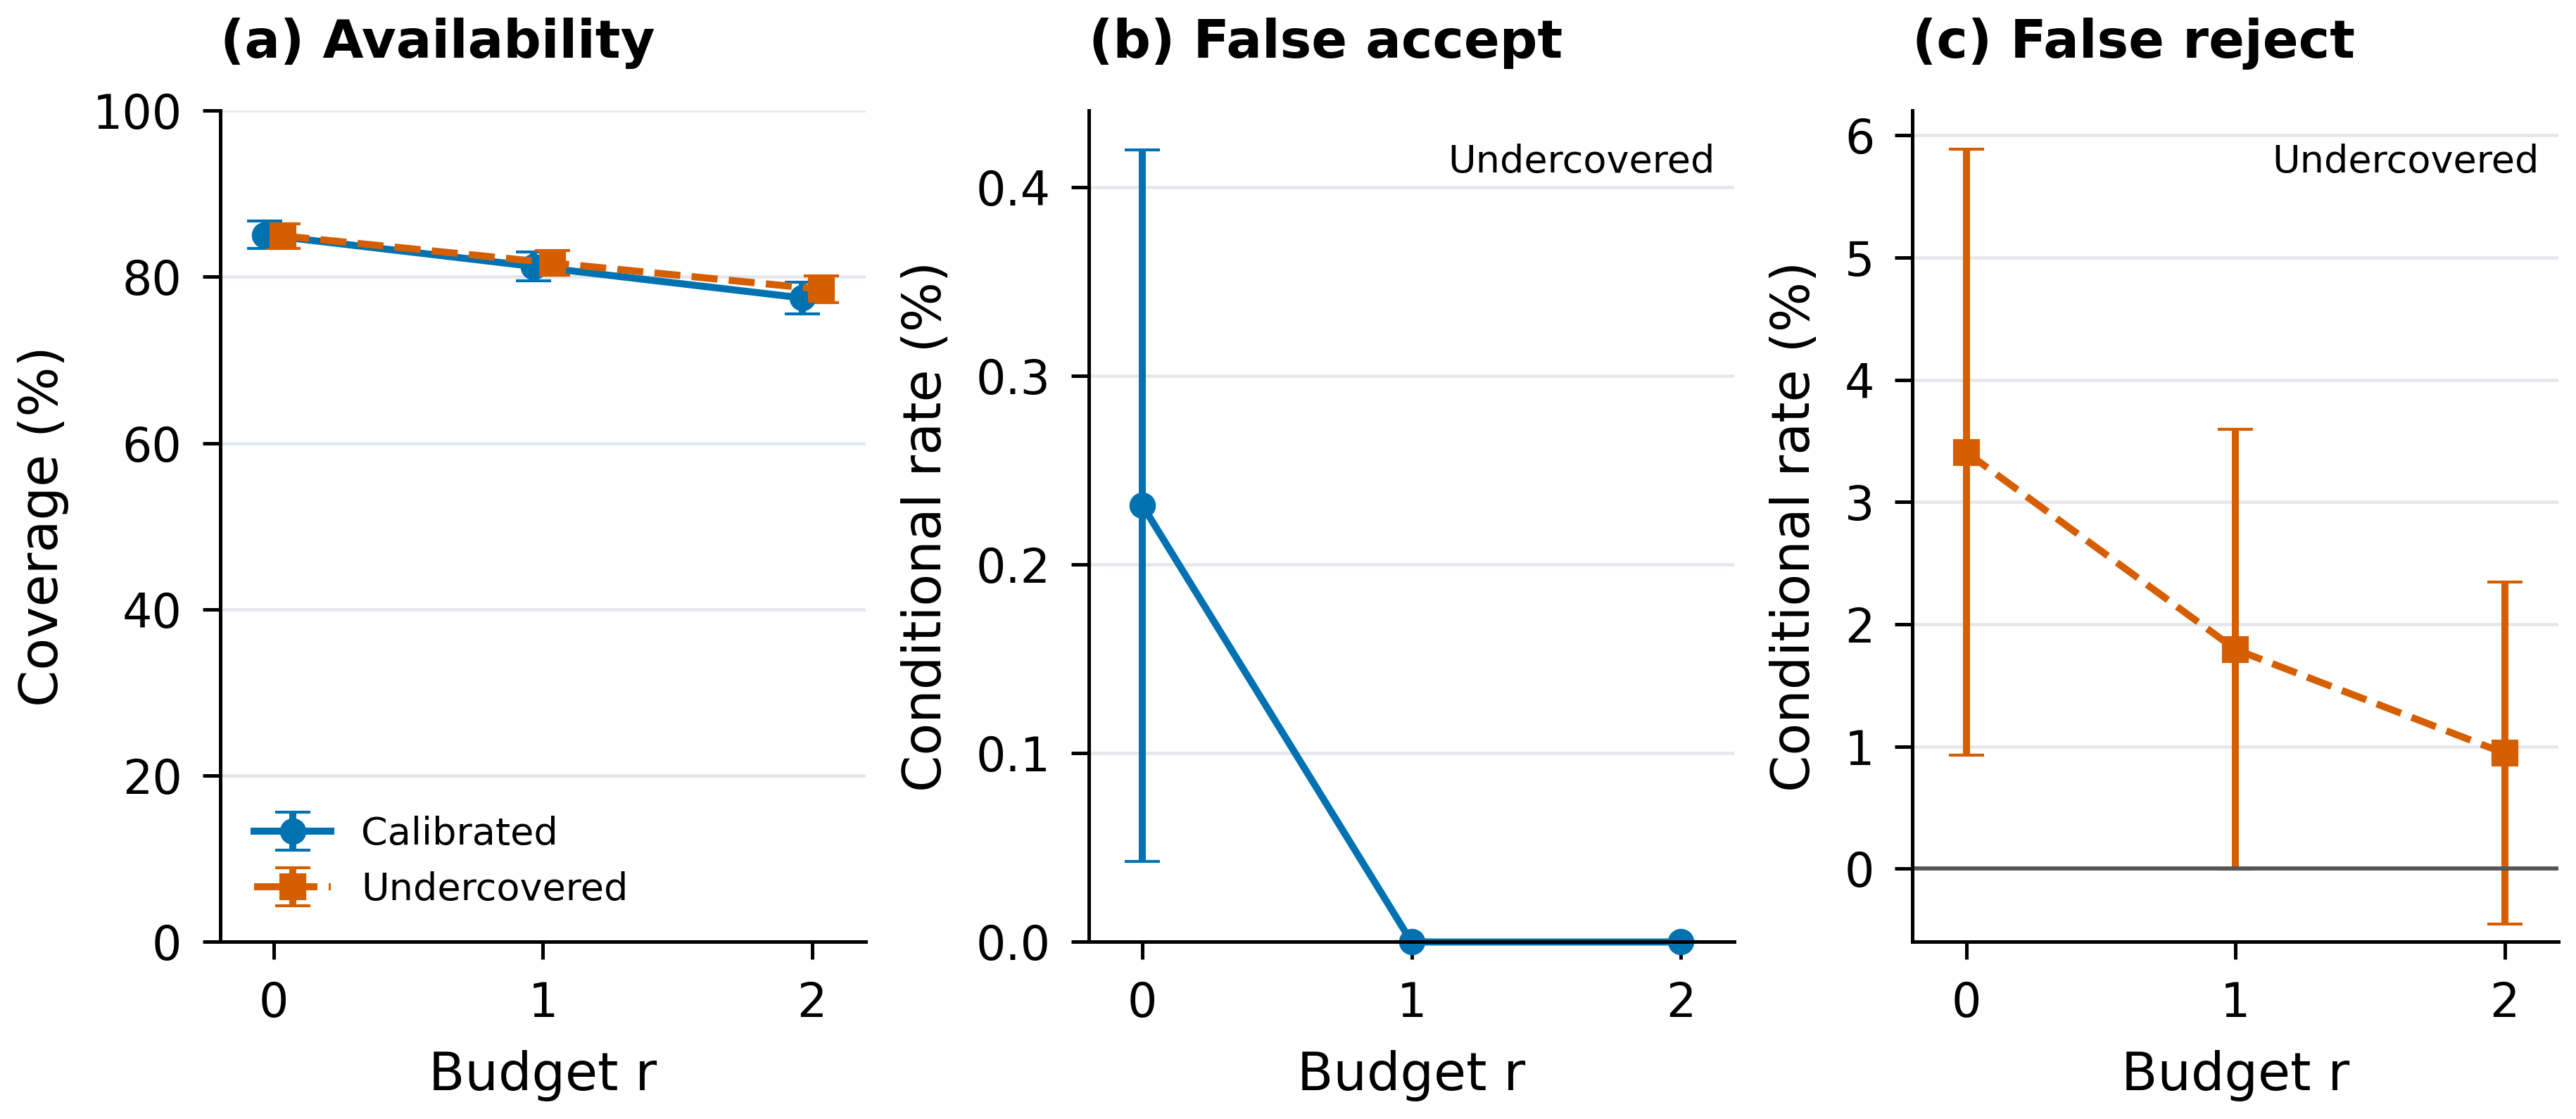
\includegraphics[width=\linewidth]{budget_tradeoff.png}
\caption{Paired ablation over the honest-miscoverage allowance $r$ for $n = 5, f = 1$: (a) decisive coverage, (b) conditional false acceptance, and (c) conditional false rejection. Points represent means and error bars indicate normal-approximation 95\% confidence intervals across 30 seeds.}\label{fig:budget}
\end{figure}